% !TEX root = thesis.tex

\chapter{The case scale}\label{ch:recurring}

In this dissertation I discuss two aspects of case competition in headless relatives.
This chapter introduces the first aspect, which concerned with the question which case wins the case competition.

It has been argued in the literature that the two competing cases always adhere a to particular case scale \citep[cf.][]{harbert1978,pittner1995,vogel2001,grosu2003,caha2019,bergsma2019}. I give the scale in \ref{ex:case-scale}.\footnote{
In the literature about headless relatives, the genitive is often discussed together with the nominative, accusative and dative \citep[cf.][]{harbert1978,pittner1995}. In this dissertation I do not discuss the genitive. I do not do so because I restrict myself to cases that appear in all possible case competition combinations. As the genitive does not fulfill that requirement, it is therefore excluded.

The genitive differs from the other cases in a particular way. That is, nominative, accusative and dative are dependents of the verb (or prepositions). Genitives can be dependents of verbs, or they can be dependents of nouns, as possessors or partitives. Most of the examples in headless relatives contain genitives that depend on nouns and not those that depend on verbs. The (genitive) possessor is also placed far away from the other three cases in \posscitet{keenan1977} relativization hierarchy.
}

\ex. \ac{nom} < \ac{acc} < \ac{dat}\label{ex:case-scale}

A case more on the right on this scale wins over a case more to the left on this scale.
This can be reformulated as follows. In a competition, accusative wins over nominative, dative wins over nominative, and dative wins over accusative. In this section I illustrate this scale with examples. When two differing cases compete, the relative pronoun always appears in the case more to the right on the case scale. It does not matter whether it is the internal or the external case.
In Section \ref{sec:pattern-rels} I give examples that illustrate that case competition in Gothic headless relative adhere to the case scale.

In the remainder of the chapter I show that the case scale is also adhered to beyond headless relatives. It also leading in case competition in numeral phrases \citep{caha2019}, which I do not discuss in this dissertation.
Besides in constructions that involve case competition, the case scale appears in other syntactic and in morphological phenomena. Section \ref{sec:impl-hier} discusses two implicational hierarchies that show the same case ordering. The hierarchies concern agreement and relativization in different languages. Section \ref{sec:case-morphology} shows that the case scale also appears in morphology. It can be observed in patterns of syncretism and in morphological containment.


\section{In headless relatives}\label{sec:pattern-rels}

In this section I give examples from case competition in Gothic headless relatives. The internal and external case take either nominative, accusative or dative case, and I show all possible combinations. All examples adhere to the case scale in \ref{ex:case-scale}.

Before I discuss examples in which the internal and external case differ and the case scale starts to play a role, I give examples in which the internal and external case match.
If the internal case and the external case are one and the same case, the relative pronoun simply surfaces in that case.

The description of Gothic is mostly based on \citep{harbert1978}. The spelling of the examples follows the Wulfila Project website.\footnote{
<http://www.wulfila.be>
} The glossing comes from the detailed tagging on that same website. The translations are my own.

Consider the example in \ref{ex:gothic-nom-nom}, in which the internal nominative case competes against the external nominative case.
The internal case is nominative, as the predicate \tit{matjan} `eat' takes nominative subjects.
The external case is nominative as well, as the predicate \tit{ga-dauþnan} `die' also takes nominative subjects.
The relative pronoun \tit{sa} `\ac{rp}.\ac{sg}.\ac{m}.\ac{nom}' appears in the internal and external case: the nominative.

\exg. ei sa -ei þis matjai, ni gadauþnai\\
\ac{comp} \ac{rp}.\ac{sg}.\ac{m}.\ac{nom} -\ac{comp} \ac{dem}.\ac{sg}.\ac{m}.\ac{gen} eat.\ac{opt}.3\ac{sg}\scsub{[nom]} not die.\ac{opt}.3\ac{sg}\scsub{[nom]}\\
`that the one, who eats of this may not die' \flushfill{Gothic, \ac{john} 6:50, after \pgcitealt{harbert1978}{337}}\label{ex:gothic-nom-nom}

Consider the example in \ref{ex:gothic-acc-acc-rep}, repeated from the introduction. In this example, the internal accusative case competes against the external accusative case.
The internal case is accusative, as the predicate \tit{arman} `pity' takes accusative objects.
The external case is accusative as well, as the predicate \tit{gaarman} `pity' also takes accusative objects.
The relative pronoun \tit{þan(a)} `\ac{rp}.\ac{sg}.\ac{m}.\ac{acc}' appears in the internal and external case: the accusative.

\exg. gaarma þan -ei arma\\
 pity.1\ac{sg}\scsub{[acc]} \ac{rp}.\ac{sg}.\ac{m}.\ac{acc} -\ac{comp} pity.1\ac{sg}\scsub{[acc]}\\
 `I pity him, whom I pity' \flushfill{Gothic, \ac{rom} 9:15, after \pgcitealt{harbert1978}{339}}\label{ex:gothic-acc-acc-rep}

Consider the example in \ref{ex:gothic-dat-dat}, in which the internal dative case competes against the external dative case.
The internal case is dative, as the predicate \tit{manwjan} `prepare' takes dative indirect objects.
The external case is dative as well, as the predicate \tit{giban} `give' also takes dative indirect objects.
The relative pronoun \tit{þaim)} `\ac{rp}.\ac{sg}.\ac{m}.\ac{dat}' appears in the internal and external case: the dative.

\exg. nist mein du giban, alja þaim -ei manwiþ was\\
{is not} 1\ac{sg}.\ac{poss}.\ac{nom} to give.\ac{inf}\scsub{[dat]} {except for} \ac{rp}.\ac{sg}.\ac{m}.\ac{dat} -\ac{comp} prepare.\ac{ptcp} be.\ac{pret}.3\ac{sg}\scsub{[dat]}\\
`it is not mine to give except for to the one, for whom it was prepared'\flushfill{Gothic, \ac{mark} 10:49, after \pgcitealt{harbert1978}{339}}\label{ex:gothic-dat-dat}

These findings are summarized as in Table \ref{tbl:summary-gothic-matching}. The left column shows the internal case between square brackets. The upper row shows the external case between square brackets. The other cells indicate the case of the relative pronoun. The top-left to bottom-right diagonal corresponds to the examples I have given so far in which the internal and external case match. The nominative marked in light gray corresponds to \ref{ex:gothic-nom-nom}, in which the internal nominative case competes against the external nominative case, and the relative pronoun surfaces in the nominative case. The accusative marked in dark gray corresponds to \ref{ex:gothic-acc-acc-rep}, in which the internal accusative case competes against the external accusative case, and the relative pronoun surfaces in the accusative case.
The unmarked dative corresponds to \ref{ex:gothic-dat-dat}, in which the internal dative case competes against the external dative case, and the relative pronoun surfaces in the dative case.

\begin{table}[ht]
 \center
 \caption{Gothic headless relatives (matching)}
 \begin{tabular}{c|c|c|c}
   \toprule
    \textsubscript{\ac{int}} \textsuperscript{\ac{ext}}
         & [\ac{nom}]
         & [\ac{acc}]
         & [\ac{dat}]
         \\ \cmidrule{1-4}
     [\ac{nom}]
         & \cellcolor{LG}{\ac{nom}}
         &
         &
         \\ \cmidrule{1-4}
     [\ac{acc}]
         &
         & \cellcolor{DG}{\ac{acc}}
         &
         \\ \cmidrule{1-4}
     [\ac{dat}]
         &
         &
         & \ac{dat}
         \\
   \bottomrule
 \end{tabular}
   \label{tbl:summary-gothic-matching}
\end{table}

In Table \ref{tbl:summary-gothic-matching}, six cells remain empty. These are the cases in which the internal and the external case differ.

I start with the competition between the accusative and the nominative. Following the case scale in \ref{ex:case-scale}, the relative pronoun appears in the accusative case and never in the nominative.

Consider the example in \ref{ex:gothic-nom-acc-rep}, repeated from the introduction. In this example, the internal accusative case competes against the external nominative case.
The internal case is accusative, as the predicate \tit{frijon} `love' takes accusative objects.
The external case is nominative, as the predicate \tit{wisan} `be' takes nominative subjects.
The relative pronoun \tit{þan(a)} `\ac{rp}.\ac{sg}.\ac{m}.\ac{acc}' appears in the internal case: the accusative. The relative pronoun is marked in bold, just as the relative clause, showing that the relative pronoun patterns with the relative clause.
Examples in which the internal case is accusative, the external case is nominative and the relative pronoun appears in the nominative case are unattested.

\exg. \tbf{þan} \tbf{-ei} \tbf{frijos} siuks ist\\
 \ac{rp}.\ac{sg}.\ac{m}.\ac{acc} -\ac{comp} love.\ac{pres}.2\ac{sg}.\scsub{[acc]} sick be.\ac{pres}.3\ac{sg}\scsub{[nom]}\\
 `the one whom you love is sick' \flushfill{Gothic, \ac{john} 11:3, adapted from \pgcitealt{harbert1978}{342}}\label{ex:gothic-nom-acc-rep}

Consider the example in \ref{ex:gothic-acc-nom-rep}, repeated from the introduction. In this example, the internal nominative case competes against the external accusative case.
The internal case is nominative, as the predicate \tit{wisan} `be' takes nominative subjects.
The external case is accusative, as the predicate \tit{ussiggwan} `read' takes accusative objects.
The relative pronoun \tit{þo} `\ac{rp}.\ac{sg}.\ac{n}.\ac{acc}' appears in the external case: the accusative. The relative pronoun is not marked in bold, just as the main clause, showing that the relative pronoun patterns with the main clause.
Examples in which the internal case is nominative, the external case is accusative and the relative pronoun appears in the nominative case are unattested.

\exg. jah þo \tbf{-ei} \tbf{ist} \tbf{us} \tbf{Laudeikaion} jus ussiggwaid\\
 and \ac{rp}.\ac{sg}.\ac{n}.\ac{acc} -\ac{comp} be.\ac{pres}.3\ac{sg}\scsub{[nom]} from Laodicea 2.\ac{pl}.\ac{nom} read.\scsub{[acc]}\\
 `and you read the one which is from Laodicea' \flushfill{Gothic, \ac{col} 4:16, adapted from \pgcitealt{harbert1978}{357}}\label{ex:gothic-acc-nom-rep}

The two examples in which the nominative and the accusative compete are shown in Table \ref{tbl:summary-gothic-nom-acc}. Within the newly filled out cells, two cases are given. The case in the bottom-left corner stands for the relative pronoun in the internal case. The case in the top-right corner stands for the relative pronoun in the external case. The grammatical examples are marked in light and dark gray. The unattested examples are preceded by an asterix and are unmarked.\footnote{
Throughout this dissertation * stands for 'not found in natural language'. For extinct languages this means that there are no attested examples. For non-extinct languages it means that the examples are ungrammatical.
}

The light gray marking corresponds to \ref{ex:gothic-nom-acc-rep}, in which the internal accusative wins the case competition over the external nominative and the relative pronoun surfaces in the accusative case. The dark gray marking corresponds to \ref{ex:gothic-acc-nom-rep}, in which the external accusative wins the case competition over the internal nominative and the relative pronoun surfaces in the accusative case. The instances of *\ac{nom} that appear in the same cells indicate that there are no examples in which the nominative and the accusative compete and the relative pronoun appears in the nominative case.

\begin{table}[ht]
 \center
 \caption{Gothic headless relatives (\ac{nom} --- \ac{acc})}
 \begin{tabular}{c|c|c|c}
   \toprule
     \diagbox[linecolor=white]{\tsc{int}}{\tsc{ext}}
         & [\ac{nom}]
         & [\ac{acc}]
         & [\ac{dat}]
         \\ \cmidrule{1-4}
     [\ac{nom}]
         & \ac{nom}
         & \diagbox[linecolor=white]{*\ac{nom}}{\colorbox{DG}{\ac{acc}}}
         &
         \\ \cmidrule{1-4}
     [\ac{acc}]
         & \diagbox[linecolor=white]{\colorbox{LG}{\ac{acc}}}{*\ac{nom}}
         & \ac{acc}
         & \diagbox[linecolor=white]{\phantom{{\tsc{xxx}}}}{\phantom{*\tsc{xxx}}}
         \\ \cmidrule{1-4}
     [\ac{dat}]
         &
         & \diagbox[linecolor=white]{\phantom{{\tsc{xxx}}}}{\phantom{*\tsc{xxx}}}
         & \ac{dat}
         \\
   \bottomrule
 \end{tabular}
   \label{tbl:summary-gothic-nom-acc}
\end{table}

I continue with the competition between the dative and the nominative. Following the case scale in \ref{ex:case-scale}, the relative pronoun appears in the dative case and never in the nominative.

Consider the example in \ref{ex:gothic-nom-dat}, in which the internal dative case competes against the external nominative case.
The internal case is dative, as the predicate \tit{fraletan} `forgive' takes dative objects.
The external case is nominative, as the predicate \tit{frijon} `love' takes nominative subjects.
The relative pronoun \tit{þamm(a)} `\ac{rp}.\ac{sg}.\ac{m}.\ac{dat}' appears in the internal case: the dative. The relative pronoun is marked in bold, just as the relative clause, showing that the relative pronoun patterns with the relative clause.
Examples in which the internal case is dative, the external case is nominative and the relative pronoun appears in the nominative case are unattested.

\exg. iþ \tbf{þamm} \tbf{-ei} \tbf{leitil} \tbf{fraletada} leitil frijod\\
 but \ac{rp}.\ac{sg}.\ac{m}.\ac{dat} -\ac{comp} little {forgive}.\ac{pass}.\ac{pres}.3\ac{sg}\scsub{[dat]} little love\scsub{[nom]}\\
 `but the one whom little is forgiven loves little' \flushfill{Gothic, \ac{luke} 7:47, adapted from \pgcitealt{harbert1978}{342}}\label{ex:gothic-nom-dat}

Consider the example in \ref{ex:gothic-dat-nom}, in which the internal nominative case competes against the external dative case.
The internal case is nominative, as the predicate \tit{wisan} `be' takes nominative subjects.
The external case is dative, as the predicate \tit{fraþjan} `think about' takes dative indirect objects.
The relative pronoun \tit{þaim} `\ac{rp}.\ac{pl}.\ac{n}.\ac{dat}' appears in the external case: the dative. The relative pronoun is not marked in bold, just as the main clause, showing that the relative pronoun patterns with the main clause.
Examples in which the internal case is nominative, the external case is dative and the relative pronoun appears in the nominative case are unattested.

\exg. þaim \tbf{-ei} \tbf{iupa} \tbf{sind} fraþjaiþ \\
 \ac{rp}.\ac{pl}.\ac{n}.\ac{dat} -\ac{comp} above be.\ac{pres}.3\ac{pl}\scsub{[nom]} {think about}.\ac{opt}.\ac{pres}.2\ac{pl}\scsub{[dat]}\\
 `think about those which are above' \flushfill{Gothic, \ac{col} 3:2, adapted from \pgcitealt{harbert1978}{339}}\label{ex:gothic-dat-nom}

The two examples in which the nominative and the dative compete are shown in Table \ref{tbl:summary-gothic-nom-dat}. The light gray marking corresponds to \ref{ex:gothic-nom-dat}, in which the internal dative wins the case competition over the external nominative and the relative pronoun surfaces in the dative case. The dark gray marking corresponds to \ref{ex:gothic-dat-nom}, in which the external dative wins the case competition over the internal nominative and the relative pronoun surfaces in the dative case. The instances of *\ac{nom} that appear in the same cells indicate that there are no examples in which the nominative and the dative compete and the relative pronoun appears in the nominative case.

 \begin{table}[ht]
  \center
  \caption{Gothic headless relatives (\ac{nom} --- \ac{dat})}
  \begin{tabular}{c|c|c|c}
    \toprule
      \diagbox[linecolor=white]{\tsc{int}}{\tsc{ext}}
          & [\ac{nom}]
          & [\ac{acc}]
          & [\ac{dat}]
          \\ \cmidrule{1-4}
      [\ac{nom}]
          & \ac{nom}
          & \diagbox[linecolor=white]{*\ac{nom}}{\ac{acc}}
          & \diagbox[linecolor=white]{*\ac{nom}}{\colorbox{DG}{\ac{dat}}}
          \\ \cmidrule{1-4}
      [\ac{acc}]
          & \diagbox[linecolor=white]{\ac{acc}}{*\ac{nom}}
          & \ac{acc}
          &
          \\ \cmidrule{1-4}
      [\ac{dat}]
          & \diagbox[linecolor=white]{\colorbox{LG}{\ac{dat}}}{*\ac{nom}}
          &
          & \ac{dat}
          \\
    \bottomrule
  \end{tabular}
    \label{tbl:summary-gothic-nom-dat}
 \end{table}

I end with the competition between the dative and the accusative. Following the case scale in \ref{ex:case-scale}, the relative pronoun appears in the dative case and never in the accusative.

Consider the example in \ref{ex:gothic-acc-dat}, in which the internal dative case competes against the external accusative case.
The internal case is dative, as the preposition \tit{ana} `on' takes dative complements.\footnote{
The example in \ref{ex:gothic-acc-dat} differs from the other examples of headless relatives. In this example, it is a preposition that assigns a particular case to the relative pronoun. So far, I have only given examples in which it is a verbal predicate that assigns a case to the relative pronoun (or the absent head). The reason for that is to keep the data set as homogenous as possible. \citet{harbert1978} reports there is no such example with the dative as internal case and the accusative as external case. My own research reaches the same conclusion. The absence of a headless relative with an internal dative case and an external accusative case (both assigned by verbal predicates) is not surprising, mainly for two reasons. First, the headless relative construction is infrequent to begin with. \citeauthor{harbert1978} reports of some case competition combinations only a single or a few occurrences.
Second, Gothic only has a few verbs that take dative complements.

There is reason to believe that this missing occurrence is due to the above mentioned reasons rather than a meaningful gap in the paradigm. Datives often appear after prepositions. There are instances in which the internal dative case is assigned by a preposition and the external accusative case is assigned by a verbal predicate. In each of these instances, the relative pronoun surfaces in the internal dative case and not in the external accusative case (as in \ref{ex:gothic-acc-dat}). For the other way around holds the same: with an accusative internal case assigned by a verbal predicate and a dative external predicate assigned by a preposition, the relative pronoun surfaces in the dative and not in the accusative. Therefore, the system that I set up later in this dissertation is able to generate the dative as internal case and accusative as external case which are both assigned by verbal predicates.
}\footnote{
\tit{Ana} `on' takes dative complements when the PP is interpreted as locational. \tit{Ana} `on' takes accusative complements when the PP is interpreted as directional. \tit{Ana þammei} `on that' in \ref{ex:gothic-acc-dat} refers to a location.
}
The external case is accusative, as the predicate \tit{ushafjan} `pick up' takes accusative objects.
The relative pronoun \tit{þamm(a)} `\ac{rp}.\ac{sg}.\ac{n}.\ac{dat}' appears in the internal case: the dative. The relative pronoun is marked in bold, just as the relative clause, showing that the relative pronoun patterns with the relative clause.
Examples in which the internal case is dative, the external case is accusative and the relative pronoun appears in the accusative case are unattested.

\exg. ushafjands \tbf{ana} \tbf{þamm} \tbf{-ei} \tbf{lag}\\
{pick up}.\ac{pres}.\ac{ptcp}\scsub{[acc]} on\scsub{[dat]} \ac{rp}.\ac{sg}.\ac{n}.\ac{dat} -\ac{comp} lie.\ac{pret}.3\ac{sg}\\
`picking up that what he lay on' \flushfill{Gothic, \ac{luke} 5:25, adapted from \pgcitealt{harbert1978}{343}}\label{ex:gothic-acc-dat}

Consider the example in \ref{ex:gothic-dat-acc}, in which the internal accusative case competes against the external dative case.
The internal case is accusative, as the predicate \tit{insandjan} `send' takes accusative objects.
The external case is dative, as the predicate \tit{galaubjan} `believe' takes dative objects.
The relative pronoun \tit{þamm(a)} `\ac{rp}.\ac{sg}.\ac{m}.\ac{dat}' appears in the external case: the dative. The relative pronoun is not marked in bold, just as the main clause, showing that the relative pronoun patterns with the main clause.
Examples in which the internal case is accusative, the external case is dative and the relative pronoun appears in the accusative case are unattested.

\exg. ei galaubjaiþ þamm \tbf{-ei} \tbf{insandida} \tbf{jains}\\
that believe.\ac{opt}.\ac{pres}.2\ac{pl}\scsub{[dat]} \ac{rp}.\ac{sg}.\ac{m}.\ac{dat} -\ac{comp} {send}.\ac{pret}.3\ac{sg}\scsub{[acc]} \ac{dem}.\ac{sg}.\ac{m}.\ac{nom}\\
`that you believe in him whom he sent' \flushfill{Gothic, \ac{john} 6:29}\label{ex:gothic-dat-acc}

The two examples in which the accusative and the dative compete are shown in Table \ref{tbl:summary-gothic-acc-dat}. The light gray marking corresponds to \ref{ex:gothic-acc-dat}, in which the internal dative wins the case competition over the external accusative and the relative pronoun surfaces in the dative case. The dark gray marking corresponds to \ref{ex:gothic-dat-acc}, in which the external dative wins the case competition over the internal accusative and the relative pronoun surfaces in the dative case. The instances of *\ac{acc} that appear in the same cells indicate that there are no examples in which the accusative and the dative compete and the relative pronoun appears in the accusative case.

 \begin{table}[ht]
  \center
  \caption{Gothic headless relatives (\ac{acc} --- \ac{dat})}
  \begin{tabular}{c|c|c|c}
    \toprule
      \diagbox[linecolor=white]{\tsc{int}}{\tsc{ext}}
          & [\ac{nom}]
          & [\ac{acc}]
          & [\ac{dat}]
          \\ \cmidrule{1-4}
      [\ac{nom}]
          & \ac{nom}
          & \diagbox[linecolor=white]{*\ac{nom}}{{\ac{acc}}}
          & \diagbox[linecolor=white]{*\ac{nom}}{{\ac{dat}}}
          \\ \cmidrule{1-4}
      [\ac{acc}]
          & \diagbox[linecolor=white]{{\ac{acc}}}{*\ac{nom}}
          & \ac{acc}
          & \diagbox[linecolor=white]{*\ac{acc}}{\colorbox{DG}{\ac{dat}}}
          \\ \cmidrule{1-4}
      [\ac{dat}]
          & \diagbox[linecolor=white]{{\ac{dat}}}{*\ac{nom}}
          & \diagbox[linecolor=white]{\colorbox{LG}{(\ac{dat})}}{*\ac{acc}}
          & \ac{dat}
          \\
    \bottomrule
  \end{tabular}
    \label{tbl:summary-gothic-acc-dat}
 \end{table}

Table \ref{tbl:summary-gothic-simple} is a simplified version of Table \ref{tbl:summary-gothic-acc-dat}. The data in the table can be divided into three sets: (1) a set of three unmarked cells in the top-left to bottom-right diagonal, (2) a set of three light gray marked cells in the bottom-left corner and (3) a set of three dark gray marked cells in the top-right corner.
The unmarked three cells in the diagonal are situations in which the internal and the external case match. They correspond to the examples \ref{ex:gothic-nom-nom}, \ref{ex:gothic-acc-acc-rep} and \ref{ex:gothic-dat-dat}.
The three cells in the bottom-left corner, marked in light gray, are the situations in which the internal case surfaces when it wins the competition. In these situations, the relative pronoun appears in the internal case. They correspond to the examples \ref{ex:gothic-nom-acc-rep}, \ref{ex:gothic-nom-dat} and \ref{ex:gothic-acc-dat}.
The three cells in the top-right corner, marked in dark gray, are the situations in which the external case surfaces when it wins the competition. In these situations, the relative pronoun appears in the external case. They correspond to the examples in \ref{ex:gothic-acc-nom-rep}, \ref{ex:gothic-dat-nom} and \ref{ex:gothic-dat-acc}.

\begin{table}[ht]
  \center
  \caption{Summary of Gothic headless relatives}
    % !TEX root = ../thesis.tex

\begin{tabular}{c|c|c|c}
  \toprule
      \textsubscript{\ac{int}} \textsuperscript{\ac{ext}}
        & [\ac{nom}]
        & [\ac{acc}]
        & [\ac{dat}]
        \\ \cmidrule{1-4}
    [\ac{nom}]
        & \ac{nom}
        & \ac{acc}
        & \ac{dat}
        \\ \cmidrule{1-4}
    [\ac{acc}]
        & \ac{acc}
        & \ac{acc}
        & \ac{dat}
        \\ \cmidrule{1-4}
    [\ac{dat}]
        & \ac{dat}
        & (\ac{dat})
        & \ac{dat}
        \\
  \bottomrule
\end{tabular}

    \label{tbl:summary-gothic-simple}
\end{table}

To sum up, case competition in headless relative is subject to the case scale, repeated in \ref{ex:case-scale-rep}.

\ex. \ac{nom} < \ac{acc} < \ac{dat}\label{ex:case-scale-rep}

If two cases compete, the dative wins over the accusative and the nominative, and the accusative wins over the nominative. In this section I gave examples from Gothic that illustrate this. As I mentioned in the introduction of this section, this case scale is not specific for Gothic, but it holds across languages (cf. see \citealt{pittner1995} for Modern and Old High German and \citealt{grosu2003,kakarikos2014} for Ancient Greek).\footnote{
Modern German differs from Gothic and the other languages in that it is subject to an additional constraint. That is, it does not allow the internal and the external case to win case competitions. Modern German only allows the internal case to do so. If the external case is more to the right on the case scale, the headless relative is ungrammatical.
This topic is the main focus of Part \ref{part:variation} of this dissertation.}

In the remainder of this chapter I show that headless relatives are not the only phenomenon where the case scale appears. Instead, it appears with more syntactic phenomena, and it is also reflected in morphology.


\section{In syntax}\label{sec:impl-hier}

In this section I discuss two additional syntactic phenomena that reflect the \ac{nom} < \ac{acc} < \ac{dat} scale. The first one is an implicational hierarchy that concerns agreement. The second one is an implicational hierarchy about relativization.


\subsection{Agreement}

Agreement can be seen as ``a systematic covariance between a semantic or formal property of one element and a formal property of another'' \citep[610]{steel1978}. Put differently, the shape of one element changes according to some properties of an element it relates to. In this section I discuss the agreement between a predicate and its arguments.

It differs per language with how many of its arguments a predicate agrees. However, it is not random with which agreement takes place. Instead, there is an implicational hierarchy that is identical to the one observed for headless relatives: \ac{nom} < \ac{acc} < \ac{dat}. First I formulate the implicational hierarchy in terms of grammatical function (following \citealt{moravcsik1978}). Later I show that a reformulation in terms of case is actually more accurate (following \citealt{bobaljik2006}).

\citet{moravcsik1978} formulated the implicational hierarchy in terms of grammatical functions subject, direct object and indirect object.\footnote{
\citet{moravcsik1978} also included adverbs on the lowest end of the hierarchy. I leave them out here, because they are not relevant for the discussion.
}
The hierarchy is schematically represented in Figure \ref{fig:agr-sub-do-io}. It should be read as follows: if a language allows the predicate to agree with the argument in a particular circle, it also allows the predicate to agree with the argument in the circle around it.

\begin{figure}[ht]
  \centering
  \begin{tabular}[b]{c}
    \toprule
  \begin{tikzpicture}
    \draw (0,1) circle (2.25);
    \draw [fill opacity=0.4, fill=LG] (0,0.5) circle (1.75);
    \draw [fill opacity=0.4, fill=DG] (0,0) circle (1.25);

    \node[] at (0,2.75) {subject};
    \node[] at (0,1.5) {direct object};
    \node[align=center] at (0,0) {indirect\\ object};
  \end{tikzpicture}\\
    \bottomrule
  \end{tabular}
  \caption{Agreement hierarchy}
  \label{fig:agr-sub-do-io}
\end{figure}

Then, there are four types of languages possible: first, a language that does not show any agreement; second, a language that shows agreement only with the subject and not with the direct and indirect object; third, a language that shows agreement with the subject and direct object but not with the indirect object; and fourth, a language that shows agreement with the subject, the direct object and the indirect object.

The implicational hierarchy holds for languages, not for sentences. That is, it is not the case that in a language of a particular type all instances of the grammatical function show agreement. To be more precise, in a language of the second type that only shows agreement with the subject, not all subjects have to show agreement. Particular types of subject, such as experiencer subjects often do not show any agreement.

Japanese is an example of a language that does not show any agreement on the predicate. An example is given in \ref{ex:japanese-agr}. The predicate \tit{okutta} `sent' does not agree with the subject \tit{Tarooga} `Taro', with the direct object \tit{nimotuo} `package' or with the indirect object \tit{Hanakoni} `Hanako'.

\exg. Taroo-ga Hanako-ni nimotu-o okutta.\\
 Taro-\ac{nom} Hanako-\ac{dat} package-\ac{acc} sent\\
 `Taro sent Hanako a package.' \flushfill{Japanese, \pgcitealt{miyagawa2004}{5}}\label{ex:japanese-agr}

German is an example of a language that shows agreement with the subject of the clause. An example is given in \ref{ex:german-agr}. The predicate \tit{gibst} `give' contains the morpheme \tit{-st}, marked in bold. This morpheme is the agreement morpheme for second person singular subjects (in the present tense). The predicate \tit{gibst} `give' agrees in person and number with the subject \tit{du} `you'. There is no agreement with the direct object \tit{das Buch} `the book' or the indirect object \tit{mir} `me'.

\exg. Du gib \tbf{-st} mir {das Buch}.\\
 you.\ac{nom} give -\ac{pres}.2\ac{sg} I.\ac{dat} {the book.\ac{acc}}\\
 `You give me the book.' \flushfill{German}\label{ex:german-agr}

Hungarian is an example of a language that shows agreement with the subject and the direct object of a clause. An example is given in \ref{ex:hungarian-agr}. The predicate \tit{adom} `give' contains the morpheme \tit{-om}, marked in bold. This is a portmonteau morpheme for a first person singular subject and a third person object agreement. The predicate \tit{adom} `give' agrees with the subject \tit{én} `I' and the direct object \tit{a könyvet} `the book'. There is no agreement with the indirect object \tit{neked} `you'. Agreement with the first person singular subject \tit{én} `I' and second person singular indirect object \tit{neked} `you.\ac{dat}.\ac{sg}' is ungrammatical, as indicated by the ungrammaticality of \tit{-lak}.

\exg. (Én) neked ad \tbf{-om}/ *-lak a könyv-et\\
 I you.\ac{dat} give -1\ac{sg}.\ac{subj}>3.\ac{obj} -1\ac{sg}.\ac{subj}>2.\ac{obj} the book-\ac{acc}\\
 `I give you the book.' \flushfill{Hungarian, András Bárány p.c.}\label{ex:hungarian-agr}

Basque is an example of a language that shows agreement with the subject, the direct object and the indirect object. Basque is an ergative-absolutive language, so in transitive clauses subjects are marked as ergative and objects are marked as absolutive. An example from the Bizkaian dialect is given in \ref{ex:basque-agr}. The stem of the auxiliary \tit{aus} combines with the morphemes \tit{d-}, \tit{-ta} and \tit{-zu}, marked in bold. The morpheme \tit{d-} is the agreement morpheme for third person singular as direct objects, which is here \tit{liburua} `the book'. The morpheme \tit{-ta} is the agreement morpheme for first person singular indirect objects, which is here \tit{niri} `me'. The morpheme \tit{-zu} is the agreement morpheme for second person singular ergative subjects, which is here \tit{zuk} `you'.

\exg. Zu-k ni-ri liburu-a emon \tbf{d} -aus \tbf{-ta} \tbf{-zu}.\\
 you-\ac{erg} I-\ac{dat} book-\ac{def}.\ac{abs} given \ac{abs}.3\ac{sg} -\ac{aux} -\ac{dat}.1\ac{sg} -\ac{erg}.2\ac{sg}\\
 `You gave me the book.' \flushfill{Bizkaian Basque, adapted from \pgcitealt{arregi2004}{45}}\label{ex:basque-agr}

Putting the languages in \posscitet{moravcsik1978} schema gives the result as shown in Figure \ref{fig:agr-sub-do-io-lang}.

 \begin{figure}[ht]
   \centering
   \begin{tabular}[b]{c}
     \toprule
   \begin{tikzpicture}
     \draw (0,1) circle (2.25);
     \draw [fill opacity=0.4, fill=LG] (0,0.5) circle (1.75);
     \draw [fill opacity=0.4, fill=DG] (0,0) circle (1.25);

     \node[] at (0,2.75) {subject};
     \node[] at (0,1.5) {direct object};
     \node[align=center] at (0,0) {indirect\\ object};

     \node[] at (2.5,3) {\footnotesize{● Japanese}};
     \node[] at (2.25,2) {\footnotesize{● German}};
     \node[] at (2,1) {\footnotesize{● Hungarian}};
     \node[] at (1.375,0) {\footnotesize{● Basque}};
   \end{tikzpicture}\\
    \bottomrule
 \end{tabular}
   \caption{Agreement hierarchy with languages}
   \label{fig:agr-sub-do-io-lang}
 \end{figure}

\citet{gilligan1987} performed a typological study among 100 genetically and areally diverse languages, which confirms the picture. The results are shown in Table \ref{tbl:agr-typo}. There are 23 languages that do not show any agreement, like Japanese. There are 31 languages that show agreement only with the subject and not with the direct and indirect object, like German. There are 25 languages that show agreement with the subject and direct object but not with the indirect object, like Hungarian. There are 23 languages that show agreement with the subject, the direct object and the indirect object, like Basque.

 \begin{table}[ht]
   \center
   \caption {Typology for agreement hierarchy}
     \begin{tabular}[t]{ccccc}
       \toprule
           \multicolumn{3}{c}{agreement with} &              &         \\
       \cmidrule{1-3}
                    & direct & indirect       & number       &         \\
           subject  & object & object         & of languages & example \\
       \cmidrule{1-3} \cmidrule{4-4} \cmidrule{5-5}
           *    & * & * & 23  & Japanese    \\
           ✔    & * & * & 31  & German     \\
           ✔    & ✔ & * & 25  & Hungarian  \\
           ✔    & ✔ & ✔ & 23  & Basque     \\
           ✔    & * & ✔ & (1) & -          \\
           {*}  & ✔ & ✔ & 0   & -          \\
           {*}  & x & * & 0   & -          \\
           {*}  & * & ✔ & 0   & -          \\
       \bottomrule
     \end{tabular}
     \label{tbl:agr-typo}
 \end{table}

So far I have discussed the implicational hierarchy in terms of grammatical function. In what follows, I discuss how it actually should be formalized in terms of the case scale that has also been observed for case competition in headless relatives.

\citet{bobaljik2006} argues that the implicational hierarchy is more accurate if it is stated in terms of case rather than grammatical function. In these situations, case seem to capture the facts for the implicational hierarchy, and grammatical function does not. It is often the case that subjects appear in the nominative case, and that direct objects appear in accusative. However, this is not always the case. Subjects can be non-nominative and direct objects can be non-accusative. \citeauthor{bobaljik2006} gives examples of two types of situations in which this is the case: non-nominative subjects in Icelandic and ergative-absolutive languages. In these situations, case seem to capture the facts for the implicational hierarchy, and grammatical function does not. I go through both situations \citeauthor{bobaljik2006} describes.

Icelandic is a language that has dative subjects. It is like German in that it only shows agreement with a single argument. If agreement takes place with the grammatical subject, it is expected that the dative subject agrees with the predicate. This is not what happens, as illustrated in \ref{ex:icelandic-dat-subj}. The dative subject \tit{morgum studentum} `many students' is plural. The sentence is ungrammatical with the predicate \tit{líka} `like' inflecting for plural as well. So, the dative subject does not agree in number with the predicate. In other words, it is not the grammatical subject that shows agreement.

\exg. *Morgum studentum líka verkið.\\
 many students.\ac{dat} like.\ac{pl} job.\ac{nom} \\
`Many students like the job.' \flushfill{\pgcitealt{harley1995}{208}}\label{ex:icelandic-dat-subj}

Instead, it is the nominative object that agrees with the verb. This is illustrated in \ref{ex:icelandic-nom-obj}. The dative subject \tit{konunginum} `the king' is singular. The nominative object \tit{ambáttir} `slaves' is plural. The predicate \tit{voru} `were' is inflected for plural, agreeing with the nominative object. This is expected if morphological case determines agreement: it is the nominative that shows agreement. The grammatical role, the fact that this nominative is an object, does not influence agreement.

\exg. Um veturinn voru konunginum gefnar ambáttir\\
In {the winter} were.\ac{pl} {the king}.\ac{sg}.\ac{dat} given slave.\ac{pl}.\ac{nom}\\
`In the winter, the king was given (female) slaves.' \flushfill{\pgcitealt{zaenen1985}{112}}\label{ex:icelandic-nom-obj}

The second type of evidence that \citeauthor{bobaljik2006} gives comes from ergative-absolutive languages. Ergative-absolutive languages differ in their alignment from nominative-accusative languages. In nominative-accusative languages, the subject of an intransitive verb (S) has the same marking as the subject of a transitive verb (A), namely nominative. The object of a transitive verb (O) has its own marking, namely accusative. This is schematically shown in \ref{fig:nom-acc-lang}.

\begin{figure}[ht]
  \centering
  \begin{tabular}[b]{c}
    \toprule
  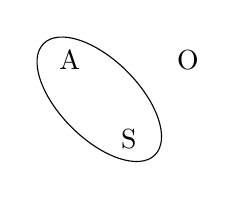
\begin{tikzpicture}
    \node[] at (0,1) {A};
    \node[] at (1.5,1) {O};
    \node[] at (0.75,0) {S};

    \draw[rotate around={45:(0.375,0.5)}] (0.375,0.5) ellipse (0.5 and 1);
  \end{tikzpicture}\\
    \bottomrule
\end{tabular}
  \caption{Nominative-accusative alignment}
  \label{fig:nom-acc-lang}
\end{figure}

In ergative-absolutive languages, the alignment is different. The subject of an intransitive verb (S) has the same marking as the object of the transitive verb (O), namely absolutive. The subject of the transitive verb (A) has its own marking, namely ergative. This is schematically shown in \ref{fig:erg-abs-lang}.

\begin{figure}[ht]
  \centering
  \begin{tabular}[b]{c}
    \toprule
  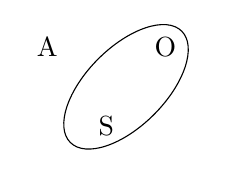
\begin{tikzpicture}
    \node[] at (0,1) {A};
    \node[] at (1.5,1) {O};
    \node[] at (0.75,0) {S};

    \draw[rotate around={135:(1,0.5)}] (1,0.5) ellipse (0.5 and 1);
  \end{tikzpicture}\\
    \bottomrule
\end{tabular}
  \caption{Ergative-absolutive alignment}
  \label{fig:erg-abs-lang}
\end{figure}

Note here that nominative-accusative languages use the same case marking for the same grammatical function (nominative for subjects, accusative for objects), but ergative-absolutive languages do not (absolutive for objects in transitive clauses or subjects in intransitive clauses, ergative for subjects in transitive clauses).

\citet{bobaljik2006} describes how absolutives and ergatives behave with respect to whether they show agreement. There are languages that show agreement with both absolutives and ergatives. There are also languages that show only agreement with absolutives. Crucially, there is no language that shows only agreement with ergatives. Absolutives are a heterogenous set with respect to grammatical function, i.e. They are subjects of intransitive verbs and objects of transitive verbs. However, with respect to showing agreement absolutives behave the same, and this behavior is different from ergatives. This indicates that it is morphological case and not grammatical function that is the decisive factor.

\citeauthor{bobaljik2006} (following \citealt{marantz2000}) combines nominative-accusative and ergative-absolutive languages in the following way: accusative and ergative are dependent cases, and nominative or absolutive are unmarked case. Reformulating Figure \ref{fig:agr-sub-do-io-lang} in terms of case instead of grammatical function gives the schema in Figure \ref{fig:agr-def-dep-dat}.

\begin{figure}[ht]
  \centering
  \begin{tabular}[b]{c}
    \toprule
  \begin{tikzpicture}
    \draw (0,1) circle (2.25);
    \draw [fill opacity=0.4, fill=LG] (0,0.5) circle (1.75);
    \draw [fill opacity=0.4, fill=DG] (0,0) circle (1.25);

    \node[] at (0,2.75) {unmarked case};
    \node[] at (0,1.5) {dependent case};
    \node[] at (0,0) {dative};

    \node[] at (2.5,3) {\footnotesize{● Japanese}};
    \node[] at (2.25,2) {\footnotesize{● German}};
    \node[] at (2,1) {\footnotesize{● Hungarian}};
    \node[] at (1.375,0) {\footnotesize{● Basque}};
  \end{tikzpicture}\\
    \bottomrule
\end{tabular}
  \caption{Agreement hierarchy (case)}
  \label{fig:agr-def-dep-dat}
\end{figure}

This formulation in terms of case rather than grammatical function works as follows for the examples I gave earlier.
First, Japanese is a language that does not show any agreement, as shown in \ref{ex:japanese-agr}. There is no agreement with the unmarked case (here the nominative), not with the dependent case (here the accusative) and not with the dative case.
Second, German is a language that shows agreement only with the unmarked case, as shown in \ref{ex:german-agr}. The morpheme \tit{-st} on the predicate agrees with the element in unmarked nominative case \tit{du} `you'. There is no agreement with the dependent accusative case or with the dative case.
Third, Hungarian is a language that shows agreement with the unmarked and the dependent case, as shown in \ref{ex:hungarian-agr}. The portmanteau morpheme \tit{-om} on the predicates agrees with the element in unmarked nominative case \tit{én} `I' and the element in dependent accusative case \tit{a könyvet} `the book'.
Last, Basque is a language that shows agreement with the unmarked, the dependent and the dative case, as shown in \ref{ex:basque-agr}. The morpheme \tit{-zu} on the auxiliary agrees with the element in dependent ergative case \tit{zuk} `you'. The morpheme \tit{d-} on the auxiliary agrees with the element in unmarked absolutive case \tit{liburua} `the book'. The morpheme \tit{-ta} on the auxiliary agrees with the element in the dative case \tit{niri} `me'.

In the languages I discuss in this dissertation, I focus on languages that have nominative as unmarked case and accusative as dependent case, so Figure \ref{fig:agr-nom-acc-dat} suffices.

\begin{figure}[ht]
  \centering
  \begin{tabular}[b]{c}
    \toprule
  \begin{tikzpicture}
    \draw (0,1) circle (2.25);
    \draw [fill opacity=0.4, fill=LG] (0,0.5) circle (1.75);
    \draw [fill opacity=0.4, fill=DG] (0,0) circle (1.25);

    \node[] at (0,2.75) {nominative};
    \node[] at (0,1.75) {accusative};
    \node[] at (0,0) {dative};
  \end{tikzpicture}\\
    \bottomrule
\end{tabular}
  \caption{Agreement hierarchy (\tsc{nom}/\tsc{acc/\tsc{dat}})}
  \label{fig:agr-nom-acc-dat}
\end{figure}

In sum, this section has shown that agreement follows the same implicational hierarchy as the case scale in headless relatives: \ac{nom} < \ac{acc} < \ac{dat}.


\subsection{Relativization}

Relativization refers to the process in which a relative clause is derived from a non-relative clause. In \ref{ex:rel-realati}, I give an example of a relative clause.

\ex. the woman, who you like\label{ex:rel-realati}

This relative clause is derived from the non-relative clause in \ref{ex:rel-non}.

\ex. You like the woman.\label{ex:rel-non}

The head of the relative clause is \tit{woman}. It precedes the relative clause. The relative pronoun \tit{who} directly follows the head. The head is no longer present in the relative clause anymore.

In \ref{ex:rel-realati}, it is the object of the clause that is relativized. It differs per language which elements can be relativized with a particular strategy. Just as the distribution was not random for agreement, it is not random which elements can be relativized. Instead, there is an implicational hierarchy that is identical to the one observed for the case scale: \ac{nom} < \ac{acc} < \ac{dat}.

\citet{keenan1977} formulated the implicational hierarchy in terms of the grammatical functions subject, direct object and indirect object.\footnote{
\citet{keenan1977} also included obliques, possessives and objects of comparison on the lowest end of the hierarchy. I leave them out here, because they are not relevant for the discussion.
}
The implicational hierarchy is schematically represented in Figure \ref{fig:rel-sub-do-io}. It should be read as follows: if a language allows a particular relativization strategy of the grammatical function in a particular circle, it also allows this relativization strategy of the grammatical function of the circle around it.

\begin{figure}[ht]
  \centering
  \begin{tabular}[b]{c}
    \toprule
  \begin{tikzpicture}
    \draw (0,1) circle (2.25);
    \draw [fill opacity=0.4, fill=LG] (0,0.5) circle (1.75);
    \draw [fill opacity=0.4, fill=DG] (0,0) circle (1.25);

    \node[] at (0,2.75) {subject};
    \node[] at (0,1.5) {direct object};
    \node[align=center] at (0,0) {indirect\\ object};
  \end{tikzpicture}\\
    \bottomrule
\end{tabular}
  \caption{Relativization hierarchy}
  \label{fig:rel-sub-do-io}
\end{figure}

There are four types of languages possible: first, a language that allows only the subject to be relativized with a particular strategy and not the direct and indirect object; second, a language that allows the subject and direct object to be relativized with a particular strategy but not the indirect object; and third, a language that allows the subject, the direct object and the indirect object to be relativized with a particular strategy.

Malagasy is an example of a language that allows subjects to be relativized using a particular strategy, but not direct and indirect objects. \ref{ex:malagasy-decl} is an example of a declarative sentence in Malagasy. It is a transitive sentence that contains the subject \tit{ny mpianatra} `the student' and the direct object \tit{ny vehivavy} `the woman'.

\exg. Nahita ny vehivavy ny mpianatra.\\
 saw the woman the student\\
 `The student saw the woman.' \flushfill{Malagasy, \pgcitealt{keenan1977}{70}}\label{ex:malagasy-decl}

In \ref{ex:malagasy-subj}, the subject from the declarative sentence, marked in bold, is relativized. The subject \tit{ny mpianatra} `the student' appears in the first position of the clause. It is followed by the invariable relativizer \tit{izay} `that'. After that, the rest of the relative clause follows, in this case \tit{nahita ny vehivavy} `saw the woman'.

\exg. \tbf{ny} \tbf{mpianatra} izay nahita ny vehivavy\\
 the student that saw the woman\\
 `the student that saw the woman' \flushfill{Malagasy, \pgcitealt{keenan1977}{70}, my boldfacing}\label{ex:malagasy-subj}

The object of \ref{ex:malagasy-decl} cannot be relativized in the same way, as shown in \ref{ex:malagasy-no-do}. Here the object \tit{ny vehivavy} `the woman', marked in bold, appears in the first position of the clause. It is again followed by the relativizer \tit{izay} `that' and the rest of the relative clause, which is here \tit{nahita ny mpianatra} `saw the student'. This example is ungrammatical.

\exg. *\tbf{ny} \tbf{vehivavy} izay nahita ny mpianatra\\
 the woman that saw the student\\
 `the woman that the student saw' \flushfill{Malagasy, \pgcitealt{keenan1977}{70}, my boldfacing}\label{ex:malagasy-no-do}

Later in this section I draw the parallel between subject and nominative, direct object and accusative and indirect object and dative \citep[after][]{caha2009}. As Malagasy does not have any overt morphological system, it does not hold that the subject corresponds to the nominative in this case.
German is another example of a language that allows subjects to be relativized using a particular strategy, but not direct and indirect object. This strategy is the participle construction \citep{keenan1977}. This strategy is a secondary strategy that exist besides the main strategy that can be used to relativize direct and indirect objects. \ref{ex:german-rel-decl} is an example of a declarative sentence in German. It is a transitive sentence that contains the subject \tit{die Frau} `the woman' and the object \tit{der Mann} `the man'.

\exg. Die Frau küsst den Mann.\\
the woman kisses the man\\
`The woman is kissing the man.' \flushfill{German}\label{ex:german-rel-decl}

The subject from the declarative in \ref{ex:german-rel-decl}, sentence \tit{die Frau} `the woman', is relativized in \ref{ex:german-rel-subj}. The predicate from the declarative clause \tit{küsst} `kisses' is turned in into the participle \tit{küssende} `kissing'. The participle appears at the end of the reduced relative clause \tit{den Mann küssende} `the man kissing'. The reduced relative clause directly precedes the noun of the subject, creating distance between the determiner \tit{die} `the' and \tit{Frau} `woman', which are both marked in bold.

\exg. \tbf{die} den Mann küssende \tbf{Frau}\\
 the man kissing woman\\
 `the woman who is kissing the man' \flushfill{German}\label{ex:german-rel-subj}

The object from the declarative sentence in \ref{ex:german-rel-decl}, \tit{den Mann} `the man', cannot be relativized like the subject, as shown in \ref{ex:german-rel-no-do}. Again, the predicate from the declarative clause \tit{küsst} `kisses' is turned in into the participle \tit{küssende} `kissing'. The participle appears at the end of the relative clause \tit{die Frau küssende} `the woman kissing'. The reduced relative clause directly precedes the noun of the object, creating distance between the determiner \tit{der} `the' and \tit{Mann} `man', which are both marked in bold. This example is ungrammatical.

\exg. *\tbf{den} die Frau küssende \tbf{Mann}\\
 the woman kissing man\\
 intended: `the man that the woman is kissing' \flushfill{German}\label{ex:german-rel-no-do}

Malay is an example of a language that has a relativization strategy for subjects and direct objects, but not for indirect objects. \ref{ex:malay-do} shows an example in which the object is relativized. The object here is \tit{ayam} `chicken', marked in bold. It is followed by the relativizer \tit{yang} `that'. After that, the rest of the relative clause \tit{Aminah sedang memakan} `Aminah is eating' follows. The same strategy works to relativize subjects, which is not illustrated with an example.

\exg. Ali bunoh \tbf{ayam} yang Aminah sedang memakan.\\
 Ali kill chicken that Aminah \ac{prog} eat\\
 `Ali killed the chicken that Aminah is eating.' \flushfill{Malay, \pgcitealt{keenan1977}{71}, my boldfacing}\label{ex:malay-do}

Indirect objects cannot be relativized using the same strategy. \ref{ex:malay-decl} is an example of a ditransitive sentence in Malay. The indirect object \tit{kapada perempuan itu} `the woman' cannot be relativized using \tit{yang}.

\exg. Ali beri {ubi kentang} itu kapada perempuan itu.\\
 Ali give potato the to woman the\\
 `Ali gave the potato to the woman.'\label{ex:malay-decl} \flushfill{Malay, \pgcitealt{keenan1977}{71}}

This is illustrated by the examples in \ref{ex:malay-no-io}. In \ref{ex:malay-no-io1}, the direct object \tit{perempuan kapada} `the woman', marked in bold, appears in the first position of the clause. It is followed by the relativizer \tit{yang} `that' and the rest of the relative clause \tit{Ali beri ubi kentang itu kapada} `Ali gave the potato to'. This example in ungrammatical.
The example in \ref{ex:malay-no-io2} differs from \ref{ex:malay-no-io1} in that the preposition \tit{kapada} `to' has been moved such that it precedes the relativizer \tit{yang} `that'. This example is ungrammatical as well, indicating this was not the reason for the ungrammaticality.

\ex.\label{ex:malay-no-io}
\ag. *\tbf{perempuan} yang Ali beri {ubi kentang} itu kapada\\
 woman that Ali give potato the to\\\label{ex:malay-no-io1}
\bg. *\tbf{perempuan} \tbf{kapada} yang Ali beri {ubi kentang} itu\\
 woman to who Ali give potato that\\\flushfill{Malay, \pgcitealt{keenan1977}{71}, my boldfacing}\label{ex:malay-no-io2}

Later in this section I draw the parallel between subject and nominative, direct object and accusative and indirect object and dative \citep[after][]{caha2009}. As Malay does not have any overt morphological system, it does not hold that the subject corresponds to the nominative and the object to the accusative.

Finnish is another example of a language that allows subjects and direct objects to be relativized using a particular strategy, but not indirect objects. This strategy places the relative clause prenominally, does not use a relativization marker, and puts the predicate in the relative clause in the non-finite form \citep{keenan1977}.

\ref{ex:finnish-rel} shows how examples of relativized subjects and direct objects.
\ref{ex:finnish-rel-sbj} is an example of a subject relative: \tit{poika} `boy' has been relativized from the clause in which it was the subject of \tit{tanssinut} `danced'. The head of the relative clause is \tit{poika} `boy', marked in bold, is preceded by the relative clause \tit{pöydällä tanssinut} `who had danced on the table'. The predicate of the relative clause appears in the non-finite form: \tit{tanssinut} `having danced'.
\ref{ex:finnish-rel-obj} is an example of a subject relative: \tit{poika} `boy' has been relativized from the clause in which it was the subject of \tit{näkemäni} `saw'. The head of the relative clause is \tit{poika} `boy', marked in bold, is preceded by the relative clause \tit{näkemäni} `that I saw'. The predicate of the relative clause appears in the non-finite form: \tit{näkemäni} `having seen'.

\ex.\label{ex:finnish-rel}
\ag. Pöydällä tanssinut \tbf{poika} oli sairas.\\
 on-table having-danced boy was sick\\
 `The boy who had danced on the table was sick.'\label{ex:finnish-rel-sbj}
\bg. Näkemäni \tbf{poika} tanssi pöydällä.\\
 I-having-seen boy danced on-table\\
 `The boy that I saw danced on the table.'\flushfill{Finnish, \pgcitealt{keenan1977}{71}}\label{ex:finnish-rel-obj}

Basque is an example of a language that has a particular relativization strategy for subjects, direct objects and indirect objects. \ref{ex:basque-decl} is an example of a declarative ditransitive sentence in Basque. The sentence contains the subject \tit{gizonak} `the man', the direct object \tit{liburua} `the book' and the indirect object \tit{emakumeari} `the woman'.

\exg. Gizon-a-k emakume-a-ri liburu-a eman dio.\\
 man-\ac{def}-\ac{erg} woman-\ac{def}-\ac{dat} book-\ac{def}.\ac{abs} give has\\
 `The man has given the book to the woman.' \flushfill{Basque, \pgcitealt{keenan1977}{72}}\label{ex:basque-decl}

A relative clause in Basque appears in the prenominal position and it is marked by the invariable marker \tit{-n}.\footnote{
Additionally, the relativized positions do not appear in verbal agreement anymore, but this not visible in the example, because they are all phonologically zero.
}
\ref{ex:basque-sub} shows the three relativizations that are derived from \ref{ex:basque-decl}.
In \ref{ex:basque-sub}, the ergative subject \tit{gizonak} `the man' from \ref{ex:basque-decl} is relativized. The head \tit{gizona} `the man', marked in bold, has lost its ergative marker \tit{-k}, and follows the relative clause \tit{makumeari liburua eman dio} `who has given the book to the woman'. The suffix \tit{-n} is attached to the relative clause.
In \ref{ex:basque-do}, the absolutive direct object \tit{liburua} `the book' from \ref{ex:basque-decl} is relativized. The head \tit{liburua} `the book', marked in bold, follows the relative clause \tit{gizonak emakumeari eman dion} `that the man has given to the woman'.\footnote{
The absolutive direct object \tit{liburua} `the book' does not have an additional overt absolutive marker, so this difference cannot be observed when it is relativized.
}
The suffix \tit{-n} is attached to the relative clause.
In \ref{ex:basque-io}, the dative indirect object \tit{emakumeari} `the woman' from \ref{ex:basque-decl} is relativized. The head \tit{emakumea} `the man', marked in bold, has lost its dative marker \tit{-ri}, and follows the relative clause \tit{gizonak liburua eman dion} `that the man has given the book to'. The suffix \tit{-n} is attached to the relative clause.

\ex.\label{ex:basque-rel}
\ag. emakume-a-ri liburu-a eman dio-n \tbf{gizon-a}\\
 woman-\ac{def}-\ac{dat} book-\ac{def}.\ac{abs} give has-\ac{rel} man-\ac{def}\\
 `the man who has given the book to the woman'\label{ex:basque-sub}
\bg. gizon-a-k emakume-a-ri eman dio-n \tbf{liburu-a}\\
 man-\ac{def}-\ac{erg} woman-\ac{def}-\ac{dat} give has-\ac{rel} book-\ac{def}\\
 `the book that the man has given to the woman'\label{ex:basque-do}
\bg. gizon-a-k liburu-a eman dio-n \tbf{emakume-a}\\
 man-\ac{def}-\ac{erg} book-\ac{def}.\ac{abs} give has-\ac{rel} woman-\ac{def}\\
 `the woman that the man has given the book to' \flushfill{Basque, \pgcitealt{keenan1977}{72}, my boldfacing}\label{ex:basque-io}

Putting the languages in the schema gives the result as shown in Figure \ref{fig:rel-sub-do-io-lang}.

 \begin{figure}[ht]
   \centering
   \begin{tabular}[b]{c}
     \toprule
   \begin{tikzpicture}
     \draw (0,1) circle (2.25);
     \draw [fill opacity=0.4, fill=LG] (0,0.5) circle (1.75);
     \draw [fill opacity=0.4, fill=DG] (0,0) circle (1.25);

     \node[] at (0,2.75) {subject};
     \node[] at (0,1.5) {direct object};
     \node[align=center] at (0,0) {indirect\\ object};

     \node[] at (2.5,2) {\footnotesize{● Malagasy/German}};
     \node[] at (2,1) {\footnotesize{● Malay/Finnish}};
     \node[] at (1.375,0) {\footnotesize{● Basque}};
   \end{tikzpicture}\\
    \bottomrule
 \end{tabular}
   \caption{Relativization hierarchy with languages}
   \label{fig:rel-sub-do-io-lang}
 \end{figure}

\citet{caha2009} argues that the implicational hierarchy is more accurate if it is stated in terms of case rather than grammatical function. The main argument comes from ergative-absolutive languages, which was also one of \posscitet{bobaljik2006} argument with the implicational hierarchy for agreement.

According to \citet{keenan1977}, ergative-absolutive languages form a counterexample to their hierarchy. It turns out that in some languages ergative subjects cannot be relativized, while absolutive subjects and absolutive objects can. This indicates that absolutive subjects and objects form a natural class to the exclusion of ergative subjects. In other words, it is not the grammatical function that is decisive, but morphological case. Dyirbal is an example of a language in which absolutive subjects and objects can be relativized, but ergative subjects cannot \pgcitep{dixon1972}{100}.

\ref{ex:dyirbal-decl} shows an intransitive and transitive sentence in Dyirbal. In the intransitive sentence in \ref{ex:dyirbal-intra}, the subject \tit{balan d̦ugumbil} `the woman' is marked absolutive. In the transtive sentence in \ref{ex:dyirbal-tra}, the subject \tit{ŋad̦a} `I' is marked ergative, and the object \tit{balan d̦ugumbil} `the woman' is marked absolutive.

\ex.\label{ex:dyirbal-decl}
\ag. balan d̦ugumbil ɲina-ɲu\\
 \ac{det}.\ac{abs} woman.\ac{abs} sit-\ac{pass}\\
 `The woman is sitting down.'\label{ex:dyirbal-intra}
\bg. ŋad̦a balan d̦ugumbil buŗa-n\\
 I.\ac{erg} \ac{det}.\ac{abs} woman.\ac{abs} see-\ac{pres}/\ac{pst}\\
 `I am watching the woman.'\flushfill{Dyirbal, \pgcitealt{dixon1972}{100}, my boldfacing}\label{ex:dyirbal-tra}

A relative clause in Dyirbal follows its head, and marks the predicate of the relative clause with the relative suffix \tit{-ŋu}.
In \ref{ex:dyirbal-abs-sub}, the absolutive subject \tit{d̦ugumbil} `woman' from \ref{ex:dyirbal-intra} is relativized. The head \tit{d̦ugumbil} `woman', marked in bold, precedes the relative clause \tit{ɲina-ŋu} `who is sitting down'. The predicate in the relative clause \tit{ɲina} `sit' is followed by the relative suffix \tit{-ŋu}.
In \ref{ex:dyirbal-abs-do}, the absolutive object \tit{d̦ugumbil} `woman' from \ref{ex:dyirbal-tra} is relativized. The head \tit{d̦ugumbil} `woman', marked in bold, precedes the relative clause \tit{ŋad̦a buŗa-ŋu} `whom I am watching'. The predicate in the relative clause \tit{buŗa} `see' is followed by the relative suffix \tit{-ŋu}.

\ex.
\ag. ŋad̦a balan \tbf{d̦ugumbil} ɲina-ŋu buŗa-n\\
 I.\ac{erg} \ac{det}.\ac{abs} woman.\ac{abs} sit-\ac{rel} see-\ac{pres}\ac{pst}\\
 `I am watching the woman who is sitting down.'\flushfill{Dyirbal, \pgcitealt{dixon1972}{100}, my boldfacing}\label{ex:dyirbal-abs-sub}
\bg. balan \tbf{d̦ugumbil} ŋad̦a buŗa-ŋu ɲina-ɲu\\
 \ac{det}.\ac{abs} woman.\ac{abs} I see-\ac{rel} sit-\ac{pass}\\
 `The woman whom I am watching is sitting down.'\flushfill{Dyirbal, \pgcitealt{dixon1972}{100}, my boldfacing}\label{ex:dyirbal-abs-do}

Ergatives (for instance the ergative subject \tit{ŋad̦a} `I' in \ref{ex:dyirbal-tra}) cannot be directly relativized. They have to be promoted to absolutives first, creating a passive-like structure. In other words, only relativization of absolutives is possible, ergatives cannot be relativized.

In conclusion, just as the agreement hierarchy, the relativization hierarchy is formalized best in terms of morphological case \citep[cf.][]{caha2009}. Reformulating Figure \ref{fig:rel-sub-do-io-lang} in terms of case instead of grammatical function gives the schema in Figure \ref{fig:rel-def-dep-dat}.

\begin{figure}[ht]
  \centering
  \begin{tabular}[b]{c}
    \toprule
  \begin{tikzpicture}
    \draw (0,1) circle (2.25);
    \draw [fill opacity=0.4, fill=LG] (0,0.5) circle (1.75);
    \draw [fill opacity=0.4, fill=DG] (0,0) circle (1.25);

    \node[] at (0,2.75) {unmarked case};
    \node[] at (0,1.5) {dependent case};
    \node[align=center] at (0,0) {dative};

    \node[] at (2.5,2) {\footnotesize{● Malagasy/German}};
    \node[] at (2,1) {\footnotesize{● Malay/Finnish}};
    \node[] at (1.375,0) {\footnotesize{● Basque}};
  \end{tikzpicture}\\
    \bottomrule
\end{tabular}
  \caption{Relativization hierarchy (case)}
  \label{fig:rel-def-dep-dat}
\end{figure}

This formulation in terms of case rather than grammatical function works as follows for the examples I gave earlier.
First, German is a language that has a particular relativization strategy for the unmarked case, as shown in \ref{ex:german-rel-subj}. The unmarked nominative case can be relativized with a reduced relative clause, but the dependent accusative case and the dative case cannot.
Second, Finnish is a language that has a particular relativization strategy for unmarked and dependent case, as shown in \ref{ex:finnish-rel}. The unmarked nominative case and the dependent accusative case can be relativized with a reduced relative clause, but the dative case cannot.
Last, Basque is a language that has a particular relativization strategy for unmarked, dependent and dative case, as shown in \ref{ex:basque-rel}. The unmarked ergative, dependent absolutive and dative case can be relativized by extraposing the head, and marking it with the invariable marker \tit{-n}.

In the languages I discuss in this dissertation, I focus on languages that have nominative as unmarked case and accusative as dependent case, so Figure \ref{fig:rel-nom-acc-dat} suffices.

\begin{figure}[ht]
  \centering
  \begin{tabular}[b]{c}
    \toprule
  \begin{tikzpicture}
    \draw (0,1) circle (2.25);
    \draw [fill opacity=0.4, fill=LG] (0,0.5) circle (1.75);
    \draw [fill opacity=0.4, fill=DG] (0,0) circle (1.25);

    \node[] at (0,2.75) {nominative};
    \node[] at (0,1.5) {accusative};
    \node[align=center] at (0,0) {dative};
  \end{tikzpicture}\\
    \bottomrule
\end{tabular}
  \caption{Relativization hierarchy (\tsc{nom}/\tsc{acc}/\tsc{dat})}
  \label{fig:rel-nom-acc-dat}
\end{figure}

In sum, this has shown that relativization follows the same implicational hierarchy as agreement and the case scale in headless relatives: \ac{nom} < \ac{acc} < \ac{dat}.


\section{In morphology}\label{sec:case-morphology}

In this chapter so far I showed that the case scale \ac{nom} < \ac{acc} < \ac{dat} can be observed in three syntactic phenomena. It appears in case competition in headless relatives, it forms the basis for the implicational hierarchy observed in agreement across languages, and the same implicational hierarchy holds for relativization strategies crosslinguistically.

In this section, I show that this same case scale can be observed in morphology. First I show that syncretism only targets continuous regions on the case scale. Then I present a language that shows morphological containment that reflects the case scale.


\subsection{Syncretism}

Syncretism refers to the phenomenon whereby two or more different functions are fulfilled by a single form \citep[cf.][]{baerman2002}. In this section I discuss literature that shows that syncretism patterns among nominative, accusative and dative are not random. Instead, they pattern along the case scale \ac{nom} < \ac{acc} < \ac{dat}.

It has widely been observed that syncretism is restricted by the linear sequence \ac{nom} --- \ac{acc} --- \ac{dat} \citep{baerman2005,caha2009,zompi2017} (and see \citealt{mcfadden2018,smith2019} for similar claims concerning root suppletion). That is, if one orders cases in this linear sequence, only contiguous regions in the sequence turn out to be syncretic.
Following that, four possible patterns are attested crosslinguistically. First, all three cases are syncretic. Second, nominative and accusative are syncretic and the dative is not. Third, the accusative and the dative are syncretic and the nominative is not. Fourth, all cases are non-syncretic.

There is one pattern that is not attested crosslinguistically. This pattern does not target continuous regions, but non-contiguous ones: nominative and dative are syncretic and accusative is not. In other words, what does not exist is an ABA pattern, in which a form B intervenes between the two identically formed As \citep{bobaljik2012}.

Table \ref{tbl:syncretisms} shows examples for each of these possible patterns.

\begin{table}[ht]
  \center
  \caption {Syncretism patterns}
    % !TEX root = ../thesis.tex

\begin{tabular}{cccccccc}
  \toprule
      \multicolumn{3}{c}{pattern}
        & \ac{nom}
        & \ac{acc}
        & \ac{dat}
        & translation
        & language \\
  \cmidrule(lr){1-3} \cmidrule(lr){4-6} \cmidrule(lr){7-7} \cmidrule(lr){8-8}
      A & A & A
        & \cellcolor{LG}jullie
        & \cellcolor{LG}jullie
        & \cellcolor{LG}jullie
        & 2\ac{pl}
        & Dutch \\
      A & A & B
        & \cellcolor{LG}sie
        & \cellcolor{LG}sie
        & ihr
        & 3\ac{sg}.\ac{f}
        & German \\
      A & B & B
        & við
        & \cellcolor{LG}okkur
        & \cellcolor{LG}okkur
        & 1\ac{pl}
        & Icelandic \\
      A & B & C
        & tú
        & teg
        & tær
        & 2\ac{sg}
        & Faroese \\
      A & B & A
        & \cellcolor{LG}
        &
        & \cellcolor{LG}
        &
        & not attested \\
  \bottomrule
\end{tabular}

  \label{tbl:syncretisms}
\end{table}

Faroese has an example of three distinct forms. The second person singular is \tit{tú} `you' for nominative, \tit{teg} `you' for accusative and \tit{tær} `you' for dative \pgcitep{lockwood1977}{70}.
Dutch has an example of a complete syncretism for nominative, accusative and dative. The second person plural pronoun is \tit{jullie} `you.\ac{pl}' is syncretic between all three cases.
Icelandic has an example of a syncretism between accusative and dative but not nominative. The first person singular plural is \tit{okkur} `us' is syncretic between accusative and dative. The nominative has a separate form: \tit{við} `we' \pgcitep{einarsson1949}{68}.
German has an example of a syncretism between nominative and accusative but not dative. The third person singular feminine \tit{sie} `she/her' is syncretic between nominative and accusative. The dative has a separate form: \tit{ihr} `her'.
Crucially, to the best of my knowledge, there is no language in which the nominative and the dative are syncretic but the accusative is not.

In sum, case syncretism follows the ordering of the case scale in headless relatives: \ac{nom} < \ac{acc} < \ac{dat}.


\subsection{Morphological case containment}

This section shows a second way in which \ac{nom} < \ac{acc} < \ac{dat} is reflected in morphology: morphological case containment \citep[cf.][]{smith2019,zompi2017,caha2010}. In some languages, the form that is used for the accusative literally contains the form that is used for the nominative. In turn, the form for the dative contains the form for the accusative. I illustrate this phenomenon with examples from Khanty.

Khanty (or Ostyak) shows morphological case containment in some of its pronouns (\pgcitealt{nikolaeva1999}{16} after \citealt{smith2019}). Three examples are given in Table \ref{tbl:cont-khanty}.

\begin{table}[ht]
  \center
  \caption {Morphological case containment in Khanty}
  \begin{tabular}{clll}
  \toprule
            & \ac{1}\ac{sg}
            & \ac{3}\ac{sg}
            & \ac{1}\ac{pl}                           \\
            \cmidrule(lr){2-2} \cmidrule(lr){3-3} \cmidrule(lr){4-4}
  \ac{nom}  & ma
            & luw
            & muŋ                                     \\
  \ac{acc}  & ma:\tbf{-ne:m}
            & luw\tbf{-e:l}
            & muŋ\tbf{-e:w}                           \\
  \ac{dat}  & ma:\tbf{-ne:m}\tbf{\tbf{-na}}
            & luw\tbf{-e:l}\tbf{\tbf{-na}}
            & muŋ\tbf{-e:w}\tbf{\tbf{-na}}       \\
  \bottomrule
  \end{tabular}
  \label{tbl:cont-khanty}
\end{table}

The nominative form for the first person singular is \tit{ma} `I'. The form for the accusative is \tit{ma:ne:m} `me'. This is the form for the nominative \tit{ma} plus the accusative marker \tit{-ne:m}. The form for the dative is \tit{ma:ne:mna} `me'. This is the form for the accusative \tit{ma:ne:m} plus the dative marker \tit{-na}. The dative formally contains the accusative, and the accusative formally contains the nominative.

The third person singular and first person plural show the same pattern. The accusative forms \tit{luwe:l} `him/her' and \tit{muŋe:w} `us' contain the nominative forms \tit{luw} and the \tit{muŋ} plus the accusative marker \tit{-e:l} or \tit{-e:w}. The dative forms \tit{luwe:lna} `him/her' and \tit{muŋe:wna} `us' contain the accusative forms \tit{luwe:l} and \tit{muŋe:w} plus the dative marker \tit{-na}. Again, the dative formally contains the accusative, which in turn contains the nominative.

Other languages that show this phenomenon are West Tocharian \citep{gippert1987} and Vlakh and Kalderaš Romani (respectively \citealt{friedman1991} and \citealt{boretzky1994}).

In sum, some languages morphologically look like \ac{nom}-\ac{acc}-\ac{dat}. This reflects the case scale \ac{nom} < \ac{acc} < \ac{dat}.

\section{Summary}

Case competition in headless relatives adheres to the case scale in \ref{ex:case-scale-sum}.

\ex. \ac{nom} < \ac{acc} < \ac{dat}\label{ex:case-scale-sum}

If the internal and external case differ, a case more on the right of the scale wins over a case more to the left on the scale.

This case scale is not only found in case competition in headless relatives. Implicational hierarchies regarding two syntactic phenomena appear across languages. The first one concerns agreement. If a language shows agreement with datives, it also shows agreement with accusatives and nominatives. If a language shows agreement with accusatives, it also shows agreement with nominatives.
The second implicational hierarchy concerns relativization. If a dative in a language can be relativized with a particular strategy, an accusative and a nominative can be too using the same strategy. If an accusative can be relativized with a particular strategy, so can a nominative with this strategy.
The case scale can also be observed in morphological patterns. First, if the cases are ordered according to the case scale, syncretism only target continuous forms, and no ABA pattern appears. Second, some languages show that the dative formally contains accusative, and that the accusative formally contains the nominative.

These phenomena show that the pattern observed in headless relatives is not something that stands on itself. The scale is a pattern that recurs across languages and across phenomena. Therefore, it should not be treated as a special process with its own stipulated rule. Instead, it should be anchored deeply into the linguistic system, such that the facts presented in this chapter can follow from it.
